%!TEX TS-program = xelatex
%!TEX encoding = UTF-8

% Unit pembaca Bahasa Indonesia untuk Methods of Algebra, Volume 1.
% Teks sumber: Copyright 2018 Wen-Wei Li, CC BY 4.0.
% Terjemahan ini dilisensikan menurut CC BY 4.0.

\documentclass[
	colors = true,
	coverpage = coverpage-id-unit-002.tex,
	fontsetup = font-setup-id.tex,
	titlesetup = titles-setup-id.tex,
	CJKthechapter = false
]{AJbook}

% Target-only Indonesian labels for source-class reader interface elements.
% The upstream AJbook.cls remains byte-identical to the frozen source closure.
\renewtcolorbox{wenxintishi}{
	breakable,
	enhanced,
	width = \textwidth,
	colback = white, colbacktitle = white,
	colframe = gray!50, boxrule=0.2mm,
	coltitle = black,
	fonttitle = \sffamily,
	attach boxed title to top left = {yshift=-\tcboxedtitleheight/2, xshift=\tcboxedtitlewidth/4},
	boxed title style = {boxrule=0pt, colframe=white},
	before skip = 0.5cm,
	top = 3mm,
	bottom = 3mm,
	title = {Petunjuk membaca}
}


\newcommand{\BuildDateID}{22 Agustus 2026}
\newcommand{\BuildDateShortID}{2026-08-22}
\AtBeginDocument{\renewcommand{\chaptermark}[1]{\markboth{Bab \thechapter\quad #1}{}}}

\usepackage{mathrsfs}
\usepackage{stmaryrd}
\SetSymbolFont{stmry}{bold}{U}{stmry}{m}{n}
\usepackage{array}
\usepackage{makecell}
\usepackage{tabularx}
\newcolumntype{Y}{>{\raggedright\arraybackslash}X}
\usepackage{tikz-cd}
\usetikzlibrary{positioning, patterns, calc, matrix, shapes.arrows, shapes.symbols}
\usepackage{braids}
\usepackage{tqft}
\usepackage{ytableau}
\usepackage{pgfplots}
\pgfplotsset{compat=1.18}
\usepackage{myarrows}
\usepackage{mycommand}

\usepackage[noautomatic]{imakeidx}
\makeindex[
	columns=2,
	program=makeindex,
	intoc=true,
	title={Indeks Istilah}]
\makeindex[
	columns=3,
	program=makeindex,
	intoc=true,
	name=sym1,
	title={Indeks Simbol}]

\usepackage{xr}
\usepackage[unicode, bookmarksnumbered]{hyperref}
% Import only frozen numbers. The empty URL prevents false links to a PDF
% that is not part of this standalone reader.
\externaldocument{unit-002-crossrefs}[]
\hypersetup{
	pdfauthor = {Wen-Wei Li},
	pdftitle = {Metode Aljabar, Jilid 1: Arsitektur Dasar - Unit 2: Aksioma ZFC},
	pdfsubject = {Terjemahan Bahasa Indonesia independen},
	pdfkeywords = {aljabar, teori himpunan, ZFC, id-ID},
	pdflang = {id-ID},
	CJKbookmarks = true}

\addbibresource{Al-jabr.bib}

\begin{document}
	\hypersetup{pageanchor=false}
	\pagestyle{empty}
	\input{coverpage-id-unit-002.tex}
	\pagestyle{fancy}
	\pagenumbering{roman}
	\setcounter{page}{1}
	\renewcommand{\contentsname}{Daftar Isi}
	\tableofcontents

	\mainmatter
	\hypersetup{pageanchor=true}
	% The guard occupies the blank source boundary after Section 1.1. A full
	% book build does not define this macro and therefore remains unchanged.
	\ifdefined\FullChapterWitness\else\def\UnitTwoZFCReader{}\fi
	% Indonesian LaTeX source for book ``Methods in Algebra''
% Copyright 2018  李文威 (Wen-Wei Li).
% Permission is granted to copy, distribute and/or modify this
% document under the terms of the Creative Commons
% Attribution 4.0 International (CC BY 4.0)
% http://creativecommons.org/licenses/by/4.0/

% To be included
\chapter{Teori himpunan}
Konsep dan operasi dasar himpunan merupakan materi matematika sekolah menengah atau mata kuliah dasar di perguruan tinggi. Bab ini bertujuan memperkukuh dan memperbarui landasan tersebut, serta melengkapinya dengan beberapa pengetahuan dasar yang kerap terlewatkan. Pokok bahasannya ialah:
\begin{compactitem}
	\item perumusan eksplisit teori himpunan aksiomatik Zermelo--Fraenkel beserta aksioma pilihan;
	\item teori ordinal dan lemma Zorn; ordinal dan rekursi transfinit jarang dibahas dalam buku teks aljabar umum, sedangkan pembuktian lemma Zorn pun sering kali sangat berputar-putar;
	\item definisi dan operasi dasar bilangan kardinal;
	\item penjelasan mengenai semesta Grothendieck, yang memungkinkan teori kategori digunakan dengan aman.
\end{compactitem}

Karena corak dan keterbatasan ruang buku ini, topik-topik tersebut hanya dapat disinggung secara ringkas. Dalam kebanyakan keadaan, matematikawan tidak perlu berhadapan langsung dengan struktur terdalam teori himpunan; hasil yang diperlukan pun dapat dianggap telah diketahui. Karena itu, pembaca boleh kembali ke bab ini hanya bila diperlukan. Namun, kajian teori kategori yang serius tidak dapat menghindari persoalan himpunan. Di pihak lain, ordinal, kardinal, dan rekursi transfinit merupakan perangkat sehari-hari bagi peneliti logika matematika dan teori himpunan. Banyak buku aljabar sama sekali tidak membahasnya, atau membahasnya dengan cara yang sukar ditembus. Mengingat metode logika---khususnya teori model \cite{Feng17}---belakangan ini makin merambah geometri, teori bilangan, dan bidang lain, pemahaman atas materi ini tentu bermanfaat. \index{teori model@teori model (model theory)}

\begin{wenxintishi}
	Pembaca harus memiliki pengetahuan paling dasar tentang teori himpunan naif. Semesta Grothendieck hanya diperlukan ketika topik yang lebih lanjut menuntut operasi tingkat tinggi pada kategori. Pembaca yang baru mulai mempelajari aljabar disarankan untuk melewati bab ini untuk sementara.
\end{wenxintishi}

\section{Ikhtisar aksioma ZFC}\label{sec:ZFC}
Apakah himpunan itu? Pada tahun 1895, G.\ Cantor memberikan penjelasan berikut \cite[p.481]{Cantor95}: ``Yang dimaksud dengan himpunan ialah suatu keseluruhan yang terbentuk dengan menghimpun sejumlah objek tertentu dan saling berbeda yang terdapat dalam persepsi atau pikiran kita; objek-objek tersebut disebut anggota himpunan itu.'' Lebih dari seabad kemudian, rumusan Cantor masih harus diakui cermat dan tepat. Meskipun demikian, memanipulasi objek-objek yang ``tertentu'' dan ``saling berbeda'' itu tanpa batas akan menimbulkan paradoks. Paradoks Russell yang termasyhur, misalnya, mempertimbangkan ``himpunan'' $\textbf{V}$ dari semua himpunan, lalu membentuk ``subhimpunan'' $\{x \in \textbf{V} : x \notin x\}$ dan memperoleh kontradiksi.\index{paradoks Russell@paradoks Russell} Pendekatan utama teori himpunan modern ialah membatasi ruang penerapan prinsip komprehensi $\left\{x : x \text{ memenuhi sifat } P\right \}$, lalu melakukan deduksi dalam logika orde pertama dengan sistem aksioma yang sesuai. Sebagai contoh, ``himpunan'' $\textbf{V}$ di atas sebenarnya bukan himpunan; paling jauh ia dapat disebut kelas.\index{teori himpunan@teori himpunan}

Buku ini menggunakan teori himpunan aksiomatik Zermelo--Fraenkel yang lazim dan menerima aksioma pilihan; sistem ini disingkat ZFC.\index{teori himpunan!ZFC} Kelak kita akan menambahkan satu aksioma mengenai kardinal besar (Hipotesis \ref{hyp:universe}). Secara sangat garis besar, ZFC dibangun di atas:
\begin{itemize}
	\item logika orde pertama, yang memuat konektif logis dan kuantor seperti $\wedge$, $\neg$, $\implies$, $\forall$, dan $\exists$, tanda kurung $(\;)$, variabel $x, y, z, \ldots$, tanda sama dengan $=$ (dipandang sebagai predikat biner), dan sebagainya; dapat ditentukan apakah suatu formula mengikuti kaidah bahasa itu---misalnya, apakah tanda kurungnya berpasangan dengan benar---dan formula yang memenuhi kaidah disebut formula terbentuk baik. Bahasa ini merupakan landasan baku logika formal; lihat \cite[Bab 2]{Feng17}.
	\item predikat biner $\in$ yang diperlukan teori himpunan, beserta aksioma \textbf{A.1} --- \textbf{A.9} yang akan dicantumkan di bawah. Jika $x \in y$, maka $x$ disebut anggota $y$. Semua objek $x,y$, dan seterusnya yang ditangani ZFC harus dipahami sebagai himpunan. Secara khusus, anggota suatu himpunan juga merupakan himpunan, sedangkan himpunan $s$ dan himpunan tunggal (\emph{singleton}) yang hanya beranggotakan $s$, yakni $\{s\}$, adalah dua hal yang berbeda.
\end{itemize}

Pada tataran logika, buku ini mengandalkan pemahaman umum. Kita tidak memakai formalisme ketat logika orde pertama, tetapi hanya menguraikan aksioma ZFC dalam bahasa informal yang digunakan matematikawan sehari-hari; seluruh deduksi formal selanjutnya dihilangkan. Rinciannya dapat ditemukan dalam buku teori himpunan mana pun, misalnya \cite{Je03,HY14}; untuk ikhtisar ringkas, lihat \cite{sep-set-theory}.
\begin{enumerate}[\bfseries {A}.1]
	\item \emph{Aksioma ekstensionalitas}: jika dua himpunan mempunyai anggota yang sama, maka kedua himpunan itu sama.

		Definisi formal himpunan kosong $\emptyset$ ialah $\{u \in X: u \neq u\}$, dengan $X$ suatu himpunan sembarang. Salah satu penerapan aksioma ekstensionalitas yang nyaris sepele ialah membuktikan bahwa $\emptyset$ tidak bergantung pada pilihan $X$, asalkan suatu himpunan memang ada. Syarat keberadaan ini dapat dijadikan ``aksioma eksistensi'' tersendiri atau dimasukkan ke dalam aksioma ketakhinggaan di bawah.
	\item \emph{Aksioma pasangan}: untuk setiap $x,y$, terdapat himpunan $\{x,y\}$ yang anggotanya tepat $x$ dan $y$.
	
		Konsep pasangan berurutan $(x,y)$ dapat direalisasikan dengan aksioma pasangan: kita dapat mendefinisikan $(x,y) := \{\{x\}, \{x,y\} \}$, lalu mendefinisikan hasil kali Kartesius $X \times Y := \{(x,y) : x \in X,\; y \in Y \}$; dengan cara yang sama dapat didefinisikan hasil kali sejumlah berhingga himpunan $X \times Y \times \cdots$. Suatu pemetaan antarahimpunan $f: X \to Y$ diidentifikasi dengan grafnya $\Gamma_f \subset X \times Y$: untuk setiap $x \in X$, irisan $\Gamma_f \cap (\{x\} \times Y)$ merupakan himpunan tunggal, yang ditulis $\{(x, f(x))\}$.
	\item \emph{Skema aksioma pemisahan}: misalkan $P$ suatu sifat himpunan, dan $P(u)$ menyatakan bahwa himpunan $u$ memenuhi sifat $P$. Untuk setiap himpunan $X$, terdapat himpunan $Y = \{u \in X : P(u) \}$.
	\item \emph{Aksioma gabungan}: untuk setiap himpunan $X$, terdapat gabungan yang bersesuaian, yaitu $\bigcup X := \{u : \exists v \in X \; \text{ sedemikian sehingga }\; u \in v\}$.
	
		Dalam aksioma ini, $X$ biasanya dipandang sebagai suatu keluarga himpunan; karena itu, $\bigcup X$ juga ditulis sebagai $\bigcup_{v \in X} v$.
	\item \emph{Aksioma himpunan kuasa}: untuk setiap himpunan $X$, seluruh subhimpunannya membentuk suatu himpunan $P(X) := \{u : u \subset X \}$.\index[sym1]{$P(X)$}
	\item \emph{Aksioma ketakhinggaan}: terdapat suatu himpunan tak hingga.

		Apakah yang dimaksud dengan himpunan tak hingga? Karakterisasi sifat ini tidak langsung tampak. Dalam bahasa formal, aksioma ketakhinggaan dapat ditulis sebagai
		\begin{gather}\label{eqn:infinity-axiom}
			\exists x \bigl[ (\emptyset \in x) \;\wedge \;\forall y \in x \left(y \cup \{y\} \in x \right)  \bigr].
		\end{gather}
		Himpunan $x$ semacam ini disebut himpunan induktif. Tujuan mengandaikan keberadaan himpunan induktif ialah mengambil darinya subhimpunan
		\[ \left\{\emptyset, \{\emptyset\}, \{  \emptyset, \{\emptyset\}\}, \{  \emptyset, \{\emptyset\}, \{  \emptyset, \{\emptyset\}\}\}, \ldots \right\}, \]
		yaitu ordinal tak hingga terhitung $\omega$ yang akan segera kita konstruksi.
	\item \emph{Skema aksioma penggantian}: misalkan $F$ suatu fungsi dengan domain berupa himpunan $X$. Maka terdapat himpunan $F(X) = \{ F(x) : x \in X\}$.
	
		Sifat $P$ dan fungsi $F$ dalam skema aksioma pemisahan dan penggantian bukan definisi biasa dalam pengertian teori himpunan, sehingga tidak menimbulkan penalaran melingkar. Keduanya sebenarnya didefinisikan oleh formula terbentuk baik dalam logika orde pertama. Sebagai contoh, fungsi $x \mapsto y$ dapat ditafsirkan sebagai formula terbentuk baik dalam logika orde pertama dengan dua variabel bebas $x,y$, katakanlah $\varphi$, yang memenuhi $\forall x\; \exists! y\; \varphi(x,y)$. Karena setiap pilihan $P$ atau $F$ menghasilkan satu aksioma yang bersesuaian, aksioma pemisahan dan penggantian masing-masing berbentuk skema aksioma.
	\item \emph{Aksioma regularitas}: setiap himpunan tak kosong memuat suatu anggota yang minimal terhadap relasi keanggotaan $\in$.
	
		Salah satu akibat penting aksioma regularitas ialah bahwa, untuk setiap himpunan $x$, tidak ada rantai keanggotaan tak hingga $x \ni x_1 \ni x_2 \ni \cdots$; khususnya, $x \notin x$. Dari sini dapat dibangun hierarki kumulatif himpunan; lihat \S\ref{sec:Grot-universe}.
	\item \emph{Aksioma pilihan}: misalkan setiap anggota himpunan $X$ merupakan himpunan tak kosong. Maka terdapat fungsi $g: X \to \bigcup X$ sedemikian sehingga $\forall x \in X, \; g(x) \in x$ (disebut fungsi pilihan).\index{aksioma pilihan@aksioma pilihan (axiom of choice)}

		Dalam aksioma pilihan, $X$ hendaknya dibayangkan sebagai suatu keluarga himpunan tak kosong. Fungsi pilihan $g(x) \in x$ berarti bahwa satu anggota dipilih dari setiap himpunan $x \in X$.
\end{enumerate}

Secara ketat, sistem formal ZFC hanya membicarakan himpunan. Beberapa teori himpunan aksiomatik yang lazim, seperti sistem NBG (von Neumann--Bernays--Gödel)\index{teori himpunan!NBG}, juga mendefinisikan konsep \emph{kelas}: setiap himpunan merupakan kelas, tetapi terdapat pula kelas yang bukan himpunan, yang disebut \emph{kelas sejati}\index{kelas sejati@kelas sejati (proper class)}. Dalam sistem ZFC, kelas hanyalah alat bantu: pada tingkat metabahasa, kelas dipahami sebagai semua himpunan yang memenuhi suatu sifat tertentu; misalnya, semua himpunan membentuk suatu kelas. Operasi pada kelas direduksi menjadi operasi pada formula terbentuk baik dalam logika orde pertama. Buku ini berusaha menghindari kelas sejati, tetapi dalam bab ini kita tetap harus menanganinya.

Gabungan $X \cup Y$, irisan $X \cap Y$, selisih $X \smallsetminus Y$, hasil kali $X \times Y$, relasi subhimpunan $X \subset Y$, fungsi, dan sebagainya merupakan konsep-konsep turunan. Pembaca tentu telah sangat mengenalnya, sehingga tidak akan diuraikan lagi. Dari konsep-konsep ini selanjutnya dapat dikonstruksi himpunan bilangan bulat taknegatif $\Z_{\geq 0}$, himpunan bilangan bulat $\Z$, himpunan bilangan rasional $\Q$, himpunan bilangan real $\R$, dan seterusnya. Dalam \S\ref{sec:order}, kita akan meninjau kembali cara mengonstruksi $\Z_{\geq 0}$ dalam teori himpunan.

Berikut ini kita uraikan secara ringkas konsep himpunan hasil bagi. Untuk setiap $n \geq 1$, pada himpunan $X$, relasi $n$-er didefinisikan sebagai suatu subhimpunan dari $X^n = \underbracket{X \times \cdots \times X}_{n\; \text{faktor}}$, yang dinyatakan dengan $R$. Dalam kebanyakan keadaan, yang dipertimbangkan ialah relasi biner; dalam hal ini, $xRy$ menyatakan $(x,y) \in R$. Suatu relasi biner $\sim$ yang memenuhi sifat-sifat berikut disebut \emph{relasi ekuivalensi}:
\begin{compactdesc}
	\item[Refleksif] $x \sim x$,
	\item[Simetris] $x \sim y \implies y \sim x$,
	\item[Transitif] $(x \sim y) \wedge (y \sim z) \implies (x \sim z)$.
\end{compactdesc}
Untuk $X$ dengan relasi ekuivalensi $\sim$ dan setiap $x \in X$, kelas ekuivalensi yang memuat $x$ ditulis $[x] := \{y \in X: y \sim x \}$. \emph{Himpunan hasil bagi}\index{himpunan hasil bagi@himpunan hasil bagi (quotient)} didefinisikan sebagai himpunan seluruh kelas ekuivalensi, yaitu $X/\sim\; := \{[x] : x \in X \}$. Dengan demikian diperoleh dekomposisi $X$ sebagai gabungan saling lepas (juga disebut partisi $X$), yakni $X = \bigcup_{[x] \in X/\sim} [x]$. Selain itu, $x \sim y$ jika dan hanya jika $x,y$ termasuk dalam subhimpunan yang sama pada partisi tersebut. Mudah dilihat bahwa relasi ekuivalensi pada $X$ berkorespondensi satu-satu dengan partisi $X$.

Kita akan menggunakan notasi teori himpunan yang lazim. Misalnya, $X \subsetneq Y$ berarti $X \subset Y$ dan $X \neq Y$; $X \sqcup Y$ menyatakan gabungan saling lepas $X$ dan $Y$; sedangkan $X^Y$ \index[sym1]{$X^Y$} menyatakan himpunan semua fungsi $f: Y \to X$. Khususnya, $2^X = P(X)$\index[sym1]{$2^X$}, dengan $2$ menyatakan suatu himpunan yang mempunyai tepat dua anggota. Kita akan menggunakan $\{\text{pt}\}$ untuk menyatakan himpunan yang mempunyai tepat satu anggota. Selanjutnya, untuk suatu himpunan indeks $I$ dan suatu keluarga himpunan $(X_i)_{i \in I}$, dapat didefinisikan
\[ \begin{array}{ll}
	\text{gabungan } \; \bigcup_{i \in I} X_i, & \text{irisan } \; \bigcap_{i \in I} X_i, \quad (I \neq \emptyset), \\
	\text{gabungan saling lepas } \; \bigsqcup_{i \in I} X_i, & \text{hasil kali } \; \prod_{i \in I} X_i.
\end{array}\]
Untuk $I=\emptyset$, gabungan dan gabungan saling lepas keduanya adalah $\emptyset$, sedangkan hasil kalinya adalah $\{\emptyset\}$. Satu-satunya definisi yang wajar bagi irisan kosong ialah kelas $\textbf{V}$ yang terdiri atas semua himpunan, tetapi hal ini tidak diperbolehkan dalam sistem ZFC.

Teori himpunan aksiomatik merupakan landasan ortodoks matematika modern. Cakupan pengungkapannya begitu luas dan taraf formalisasinya begitu tinggi sehingga matematika itu sendiri dapat menjadi objek penelitian matematika. Pertanyaan seperti apakah yang dimaksud dengan bukti, apakah suatu pernyataan dapat dibuktikan, dan apakah suatu sistem aksioma konsisten (bebas kontradiksi), semuanya dapat diberi kandungan matematis yang jelas; bidang penelitian semacam ini secara kolektif disebut metamatematika\index{metamatematika@metamatematika (metamathematics)}. Definisi, argumen, dan praktik matematika lain yang biasanya disampaikan dalam bahasa alami ``pada prinsipnya'' dapat ditulis ulang dalam bahasa formal ZFC atau teori himpunan aksiomatik lainnya, sehingga perumusan dan verifikasinya memperoleh landasan yang kukuh. Entah itu suatu keberuntungan atau kemalangan, selama ini landasan tersebut tak lebih daripada suatu sikap pada tataran prinsip: bahkan perumusan formal teorema teori himpunan yang tampak sederhana pun sering sangat bertele-tele, apalagi jika harus diverifikasi atau bahkan dipahami secara manual. Namun, seiring kemajuan berkelanjutan dalam logika simbolik, teori komputasi, dan teknologi terkait, keadaan ini berangsur-angsur berubah. Hasil-hasil seperti teorema empat warna, teorema bilangan prima, dan dugaan Kepler kini telah memiliki verifikasi formal, dan penerapan metode formal tidak terbatas pada matematika. Gagasan-gagasan di luar teori himpunan, seperti teori tipe, tampaknya diperlukan untuk tujuan ini, atau setidaknya memberikan penyederhanaan yang sangat besar. Satu hal dapat dipastikan: seiring teori dan teknologi berkembang bersama, pemahaman manusia mengenai landasan maupun praktik matematika akan terus ditulis ulang.
\ifdefined\UnitTwoZFCReader\expandafter\endinput\fi
\section{Struktur Urutan dan Ordinal}\label{sec:order}
Menurut pandangan Bourbaki, struktur urutan, bersama struktur topologis dan struktur aljabar, membentuk tiga struktur induk utama matematika. Berikut ini diperkenalkan secara berurutan konsep urutan parsial, urutan total, dan urutan baik.

\begin{definition}\label{def:partial-order}\index{himpunan terurut parsial@himpunan terurut parsial (partially ordered set/poset)}\index{himpunan praterurut@himpunan praterurut (pre-ordered set)}
	Suatu \emph{himpunan terurut parsial} (atau \emph{poset}) adalah data $(P, \leq)$, dengan $P$ suatu himpunan dan $\leq$ suatu relasi biner pada $P$ (urutan parsial), yang memenuhi
	\begin{compactdesc}
		\item[Refleksivitas] $\forall x \in P, \; x \leq x$;
		\item[Transitivitas] $(x \leq y) \wedge (y \leq z) \implies x \leq z$;
		\item[Antisimetri] $(x \leq y) \wedge (y \leq x) \implies x=y$.
	\end{compactdesc}
	Struktur dengan refleksivitas dan transitivitas saja disebut \emph{himpunan praterurut}. Untuk himpunan praterurut, peta yang memenuhi $x \leq y \implies f(x) \leq f(y)$ disebut \emph{peta pelestari urutan}.

	Pada umumnya, $x < y$ digunakan untuk menyatakan $x \leq y$ dan $x \neq y$. Makna simbol $\geq$ dan $>$ jelas dengan sendirinya. Selanjutnya, ketika membicarakan himpunan terurut parsial, relasi $\leq$ di dalamnya sering dihilangkan dari notasi.
\end{definition}

Misalkan $P, Q$ himpunan terurut parsial. Jika peta $\phi: P \to Q$ memenuhi $(x < x') \implies (\phi(x) < \phi(x'))$, maka $\phi$ disebut naik tegas. Jika $\phi: P \to Q$ merupakan bijeksi dan $\phi, \phi^{-1}$ keduanya merupakan peta pelestari urutan, maka $\phi$ disebut isomorfisme antara himpunan terurut parsial $P,Q$. Kelas isomorfisme dari suatu himpunan terurut parsial disebut \emph{tipe urutan}. Setiap subhimpunan dari himpunan terurut parsial mewarisi struktur urutan parsial yang alami.

\begin{definition}\label{def:max-sup}\index{elemen maksimal@elemen maksimal (maximal element)}\index{batas atas@batas atas (upper bound), supremum}\index{batas bawah@batas bawah (lower bound), infimum}
	Misalkan $P' \subset P$, dengan $P$ suatu himpunan praterurut.
	\begin{compactitem}
		\item Elemen $x \in P$ disebut elemen maksimal dari $P$ jika tidak terdapat $y \in P$ yang memenuhi $x < y$;
		\item Elemen $x \in P$ disebut batas atas dari $P'$ jika $x' \leq x$ untuk setiap $x' \in P'$;
		\item Elemen $x \in P$ disebut supremum dari $P'$ jika $x$ merupakan batas atasnya dan $x \leq y$ untuk setiap batas atas $y$.
	\end{compactitem}
	Dengan cara serupa dapat didefinisikan elemen minimal, batas bawah, dan infimum, cukup dengan mengganti $\leq$ di atas dengan $\geq$. Untuk himpunan terurut parsial $P$, antisimetri memastikan bahwa supremum atau infimum suatu subhimpunan $P'$, jika ada, bersifat unik; masing-masing dinotasikan dengan $\sup P'$ dan $\inf P'$. \index[sym1]{sup@$\sup$}\index[sym1]{inf@$\inf$}
\end{definition}

\begin{definition}\label{def:filtrant-poset}\index{poset terarah ke atas@poset terarah ke atas (filtered poset)}
	Jika himpunan terurut parsial $P$ tidak kosong dan, untuk setiap $x,y \in P$, subhimpunan $\{x,y\}$ mempunyai batas atas, maka $P$ disebut \emph{poset terarah ke atas} (\emph{filtered poset}).
\end{definition}

\begin{definition}\index{himpunan terurut total@himpunan terurut total (totally ordered set)}\index{rantai@rantai (chain)}
	Jika setiap pasangan elemen $x,y$ dalam himpunan terurut parsial $P$ dapat dibandingkan (yakni, $x \leq y$ atau $y \leq x$), maka $P$ disebut \emph{himpunan terurut total}. Himpunan terurut total juga disebut \emph{himpunan terurut linear} atau \emph{rantai}.
\end{definition}
Jelas bahwa setiap himpunan terurut total terarah ke atas.

Sesekali kita juga akan membicarakan urutan atau urutan total pada kelas tertentu, beserta batas atas, batas bawah, dan sebagainya; contohnya ialah kelas ordinal $\textbf{On}$ yang akan dibahas di bawah. Definisinya sama seperti di atas.

\begin{definition}[G.\ Cantor]\label{def:well-ordered}\index{himpunan terurut baik@himpunan terurut baik (well-ordered set)}
	Himpunan terurut total $P$ disebut \emph{himpunan terurut baik} jika memenuhi sifat berikut: setiap subhimpunan tak kosong dari $P$ mempunyai elemen minimal.
\end{definition}

\begin{example}
	Untuk sebarang himpunan $X$, himpunan kuasa $P(X)$, terhadap relasi inklusi $\subset$, merupakan poset terarah ke atas, tetapi pada umumnya tidak terurut total. Himpunan bilangan bulat taknegatif $\Z_{\geq 0}$ dan himpunan bilangan real $\R$, yang akan dikonstruksi kemudian, keduanya mempunyai struktur urutan total baku; di antaranya, $\Z_{\geq 0}$ jelas terurut baik, sedangkan $\R$ tidak.
\end{example}

\begin{lemma}\label{prop:wellorder-automorphism}
	Misalkan $P$ himpunan terurut baik dan peta $\phi: P \to P$ naik tegas. Maka $\phi(x) \geq x$ untuk setiap $x \in P$. Khususnya:
	\begin{inparaenum}[(i)]
		\item $P$ tidak mempunyai automorfisme taktrivial,
		\item untuk setiap $x \in P$, tidak terdapat isomorfisme dari $P$ ke $P_{< x} := \{y \in P : y < x \}$.
	\end{inparaenum}
\end{lemma}
Subhimpunan berbentuk $P_{< x}$ mewarisi urutan baik dari $P$ dan disebut sebuah \emph{segmen awal} dari $P$.
\begin{proof}
	Andaikan himpunan $P_0 := \{x \in P : \phi(x) < x \}$ tidak kosong. Untuk setiap $z \in P_0$, karena $\phi$ naik tegas, diperoleh $\phi(\phi(z)) < \phi(z)$. Mengambil $z$ sebagai elemen minimal dari $P_0$ menghasilkan kontradiksi. Pernyataan pertama pun terbukti.

	Untuk (i), terapkan pernyataan pertama kepada $\phi$ dan $\phi^{-1}$ sehingga diperoleh $\forall x \; \phi(x)=x$. Untuk (ii), suatu isomorfisme $\phi: P \to P_{< x}$ tentu merupakan peta naik tegas dari $P$ ke dirinya sendiri dan memenuhi $\phi(x) < x$, bertentangan dengan hasil sebelumnya.
\end{proof}

Gagasan awal mengenai ordinal ialah tipe urutan dari suatu himpunan terurut baik. Jika pendekatan ini diikuti, tipe urutan tersebut harus dipandang sebagai kelas, bukan himpunan. Dengan demikian, membicarakan kelas semua ordinal $\textbf{On}$ sama dengan menangani ``kelas dari kelas'', yang jelas agak rumit. Untungnya, dari setiap tipe urutan baik kita dapat memilih sebuah himpunan terurut baik yang baku sehingga memperoleh deskripsi yang lebih tepat. Untuk itu diperlukan definisi von Neumann berikut.
\begin{definition}\label{def:ordinal}\index{ordinal@ordinal}
	Jika setiap elemen suatu himpunan $\alpha$ merupakan subhimpunan dari $\alpha$ (dengan kata lain, $\alpha \subset P(\alpha)$), maka $\alpha$ disebut \emph{transitif}. Jika relasi $x < y \stackrel{\text{def}}{\iff} x \in y$ memberikan urutan baik pada himpunan transitif $\alpha$, maka $\alpha$ disebut \emph{ordinal}.
\end{definition}

Jelas bahwa $\emptyset$ merupakan ordinal. Jika $\alpha$ merupakan ordinal, maka $\alpha \sqcup \{\alpha\}$ juga demikian. Teori lengkap ordinal dapat ditemukan dalam \cite[\S 2]{Je03} atau \cite[Bab 4]{HY14}; berikut ini hanya dirangkum beberapa sifat penting. Hubungan antara ordinal dan tipe urutan baik diberikan dalam Proposisi \ref{prop:ordinal-ordertype}.

\begin{lemma}\label{prop:ordinal-property}
	Ordinal memenuhi sifat-sifat berikut.
	\begin{compactenum}[(i)]
		\item Jika $\alpha$ merupakan ordinal dan $\beta \in \alpha$, maka $\beta$ juga merupakan ordinal.
		\item Bagi setiap pasangan ordinal $\alpha, \beta$, jika $\alpha \subsetneq \beta$, maka $\alpha \in \beta$.
		\item Bagi setiap pasangan ordinal $\alpha, \beta$, berlaku $\alpha \subset \beta$ atau $\beta \subset \alpha$.
	\end{compactenum}
\end{lemma}
\begin{proof}
	Pertama, kita buktikan (i). Dari transitivitas $\alpha$ diperoleh $\beta \subset \alpha$, dan $(\beta, \in)$ juga merupakan himpunan terurut baik. Selanjutnya, kita buktikan bahwa $\beta$ transitif: misalkan $\tau \in \beta \subset \alpha$; cukup dibuktikan bahwa $x \in \tau \implies x \in \beta$. Karena $\in$ memberikan struktur urutan pada $\alpha$, dari $x \in \tau \in \beta$ diperoleh $x \in \beta$.

	Untuk (ii), tuliskan $<$ bagi $\in$ dan ambil $\gamma$ sebagai elemen minimal dari $(\beta \smallsetminus \alpha, <)$. Kita akan menunjukkan bahwa $\alpha = \{x \in \beta : x < \gamma \}$, sedangkan himpunan di ruas kanan tidak lain adalah $\gamma$. Inklusi $\supset$ mengikuti minimalitas elemen tersebut. Untuk inklusi $\subset$, ambil $y \in \alpha \subset \beta$. Pertama, $\gamma = y$ tidak mungkin; selanjutnya, dari transitivitas $\alpha$ diperoleh $y \subset \alpha$, sehingga kemungkinan $\gamma < y$ juga tersingkir. Jadi $y < \gamma$.

	Untuk (iii), jelas bahwa $\gamma := \alpha \cap \beta$ juga merupakan ordinal. Kita akan menunjukkan bahwa $\gamma = \alpha$ atau $\gamma = \beta$ harus berlaku. Jika tidak, hasil di atas memberikan $\gamma \in \alpha$ dan $\gamma \in \beta$, sehingga $\gamma \in \gamma$; dengan kata lain, $\gamma < \gamma$ dalam himpunan terurut parsial $(\alpha, \leq)$. Ini bertentangan dengan makna $<$, yakni $\leq$ tetapi $\neq$.
\end{proof}

Lemma tersebut langsung memberikan akibat berikut.
\begin{theorem}\label{prop:On-wellorder}
	Definisikan $\textbf{On}$ sebagai kelas yang terdiri atas semua ordinal. \index[sym1]{$\textbf{On}$}
	\begin{compactitem}
		\item Untuk ordinal, definisikan $\beta < \alpha$ jika dan hanya jika $\beta \in \alpha$. Relasi ini memberikan urutan total pada $\textbf{On}$, dan untuk setiap ordinal $\alpha$ berlaku $\alpha = \{ \beta : \beta < \alpha \}$.
		\item Jika $C$ merupakan kelas yang terdiri atas ordinal dan $C \neq \emptyset$, maka $\inf C := \bigcap C$ juga merupakan ordinal, dan $\inf C \in C$; selain itu, $\alpha \sqcup \{\alpha\} = \inf\{ \beta: \beta > \alpha \}$.
		\item Jika $S$ merupakan himpunan yang terdiri atas ordinal dan $S \neq \emptyset$, maka $\sup S := \bigcup S$ juga merupakan ordinal.
	\end{compactitem}
\end{theorem}
Dari sini, $\beta < \alpha$ menyiratkan bahwa $\beta$ merupakan segmen awal dari $\alpha$. Sifat $\alpha = \{\beta: \beta < \alpha \}$ adalah kunci untuk memahami konstruksi ordinal.

Untuk suatu ordinal $\alpha$, tetapkan $\alpha + 1 := \alpha \sqcup \{\alpha\} > \alpha$, yang disebut \emph{penerus} $\alpha$; ini merupakan ordinal terkecil yang lebih besar daripada $\alpha$. Jika $\alpha$ bukan penerus dari ordinal mana pun, mudah dilihat bahwa $\alpha = \sup\{\beta: \beta < \alpha\}$. Ordinal $\alpha$ seperti ini disebut \emph{ordinal limit}\index{ordinal!ordinal limit (limit ordinal)}. Dengan konvensi bahwa $\sup$ dari himpunan kosong bernilai $\emptyset$, ``ordinal nol'' $\emptyset$ merupakan ordinal limit.

\begin{proposition}\label{prop:Ord-class}
	Kelas ordinal $\textbf{On}$ merupakan kelas sejati.
\end{proposition}
\begin{proof}
	Hasil sebelumnya menunjukkan bahwa jika $\textbf{On}$ merupakan himpunan, maka $\sup(\textbf{On})$ terdefinisi, dan ordinal $\sup(\textbf{On}) + 1$ akan lebih besar daripada setiap ordinal, termasuk dirinya sendiri!
\end{proof}
Hal ini disebut paradoks Burali--Forti (1897)\index{paradoks Burali--Forti@paradoks Burali--Forti}; paradoks tersebut muncul lebih dahulu daripada paradoks Russell (1902), meskipun pengaruh paradoks yang terakhir lebih besar.

\begin{example}[Konstruksi ordinal tak hingga $\omega$] \index[sym1]{omega@$\omega$}\leavevmode\par
	Tinjau ordinal $0 := \emptyset$. Dengan mengambil penerus berulang kali, diperoleh ordinal
	\[ 1 := 0 + 1, \quad 2 := 1+1, \quad 3=2+1, \ldots \]
	dan seterusnya. Sekarang kita hendak mendefinisikan ordinal limit tak nol terkecil $\omega$. Jika ordinal seperti itu ada, ia harus memuat semua $0,1,2, \ldots$, dan sesungguhnya ordinal-ordinal itulah seluruh anggotanya. Langkah pertama ialah membuktikan keberadaan ordinal limit tak nol. Ingat kembali konsep himpunan induktif dalam aksioma ketakhinggaan \textbf{A.6}. Jika $x$ merupakan himpunan induktif, ambil $\alpha := \{y \in x : y \subset x, \; y \in \textbf{On} \}$. Langsung dari definisi dapat diverifikasi sifat-sifat berikut:
	\begin{inparaenum}[(a)]
		\item $\emptyset \in \alpha$, sehingga $\alpha$ tidak kosong,
		\item $\alpha$ merupakan ordinal,
		\item $y \in \alpha \implies y + 1 \in \alpha$, sehingga $\alpha$ memang merupakan ordinal limit.
	\end{inparaenum}
	Ambil ordinal $\omega := \inf\{ \text{ordinal limit tak nol} \}$. Inilah ordinal yang dicari. Ordinal $n$ yang memenuhi $n < \omega$ disebut \emph{ordinal berhingga}.

	Hingga isomorfisme, ordinal $\omega = \{n : n=0, 1, \ldots \}$ tidak lain ialah himpunan terurut baik $\Z_{\geq 0}$ yang kita kenal secara intuitif. Konstruksi ini juga dapat dipandang sebagai cara mendefinisikan himpunan bilangan bulat taknegatif dengan bertolak dari himpunan kosong dalam kerangka ZFC. Lebih tepatnya, $\omega$, bersama operasi penerus pada elemen-elemennya $n \mapsto n+1$, memenuhi aksioma aritmetika Peano (lihat \cite[Bab 0, \S 2]{DN00}); itulah seluruh sifat yang kita perlukan untuk bekerja dengan bilangan bulat dalam praktik. Teorema \ref{prop:transfinite-induction} akan membahas salah satu sifat kunci tersebut: induksi matematika.
\end{example}

\section{超穷递归及其应用}
定理 \ref{prop:On-wellorder} 表明真类 $\textbf{On}$ 对 $\leq$ 也有良序性质: 任何由序数构成的类都有极小元. 这立即导向以下结果.
\begin{theorem}[超穷归纳法]\label{prop:transfinite-induction} \index{chaoqiongguinafa@超穷归纳法 (transfinite induction)}
	令 $C$ 为一个由序数构成的类. 假设
	\begin{compactenum}[(i)]
		\item $0 \in C$,
		\item $\alpha \in C \implies \alpha+1 \in C$,
		\item 设 $\alpha$ 为极限序数, 若对每个 $\beta < \alpha$ 皆有 $\beta \in C$, 则 $\alpha \in C$,
	\end{compactenum}
	那么 $C = \textbf{On}$. 如果仅考虑小于某 $\theta$ 的序数而非 $\textbf{On}$ 整体, 断言依然成立.
\end{theorem}
\begin{proof}
	设若不然, 取不在 $C$  中的最小序数 $\alpha \neq 0$, 无论它是后继或极限序数都导致矛盾.
\end{proof}
\begin{remark}
	回忆到 $\theta = \{\alpha \in \textbf{On}: \alpha < \theta \}$. 如取 $\theta = \omega$ 则得到经典的数学归纳法, 此时不涉及情况 (iii).
\end{remark}

定理 \ref{prop:transfinite-induction} 常用以递归地构造一列以序数枚举的数学对象, 它基于某规则 $G$ 如下:
\begin{compactdesc}
	\item[第零项] $a_0 = G(0)$ 给定,
	\item[后继项] 设 $\alpha = \beta+1$, 已知 $a_\beta$, 则可以确定 $a_\alpha = a_{\beta + 1} = G(a_\beta)$,
	\item[极限项] 设 $\alpha$ 是极限序数, 已知 $\{a_\beta : \beta < \alpha \}$, 则可以确定 $a_\alpha = G(\{a_\beta : \beta < \alpha \})$.
\end{compactdesc}
不难想象这将唯一确定一列集合 $a_\alpha$, 兹改述并证明如下. 考虑函数 $G: \textbf{V} \to \textbf{V}$, 虽然 $\textbf{V}$ 是真类, 然而如早先所述, $G$ 可以诠释为一阶逻辑中的某类公式而不影响以下操作. 引入 $\theta$-列的概念: 这是指函数 $a: \theta \to \textbf{V}$, 亦可理解为形如 $\{a_\alpha : \alpha < \theta \}$ 的列.

\begin{theorem}[超穷递归原理]
	对任意序数 $\theta$, 存在唯一的 $\theta$-列 $a$ 使得 $\alpha < \theta \implies a(\alpha) = G(a|_\alpha)$. 特别地, 存在唯一的函数 $a: \textbf{On} \to \textbf{V}$ 使得对每个序数 $\alpha$ 皆有 $a(\alpha) = G(a|_\alpha)$.
\end{theorem}
几点说明:
\begin{inparaenum}[(a)]
	\item 替换公理模式 \textbf{A.7} 确保函数限制 $a|_\alpha$ 可以按寻常方法等同于集合 $\{ (\beta, a(\beta)) : \beta \in \alpha \}$, 故 $G$ 对之可以取值;
	\item 我们将函数限制 $a|_0$ 理解为空集 $0$, 故按定义 $a(0) = G(0)$;
	\item 定理前半段只要求 $G$ 对形如 $\alpha \to \textbf{V}$ 的函数有定义, 其中 $\alpha < \theta$.
\end{inparaenum}
\begin{proof}
	第一步, 若 $\theta$-列 $a, a'$ 皆满足所示性质, 我们断言 $\alpha < \theta$ 蕴涵 $a(\alpha) = a'(\alpha)$, 如是则 $a=a'$: 这对 $\alpha=0$ 已知; 设若这对所有 $\beta < \alpha$ 成立, 那么 $a|_\alpha = a'|_\alpha$ 故 $a(\alpha) = a'(\alpha)$; 应用定理 \ref{prop:transfinite-induction} 遂得以上断言.
	
	第二步是 $\theta$-列 $a$ 的存在性. 当 $\theta=0$ 时为显然. 今设 $\theta > 0$, 并且对任意 $\xi < \theta$, 所求 $\xi$-列 $a[\xi]$ 皆存在, 则由替换公理模式知 $a[\xi]$ 确实是集合间的映射; 由第一步可将诸 $a[\xi]$ 拼接为定义在 $\theta$ 上的函数 $a$ 使得 $a|_\xi = a[\xi]$, 而且使性质 $\alpha < \theta \implies a(\alpha) = G(a|_\alpha)$ 成立, 这是容易的.
	
	最后, 由于 $\textbf{On}$ 无极大元, 根据前两步可以唯一地定义 $a: \textbf{On} \to \textbf{V}$.
\end{proof}

借助超穷递归原理, 能对序数定义类似于非负整数的运算如次. 以下在情形 (iii) 总假设 $\beta$ 是极限序数:
\begin{itemize}
	\item 加法: \begin{inparaenum}[(i)] \item $\alpha + 0 := \alpha$,  \item $\alpha + (\beta + 1) = (\alpha + \beta) + 1$, \item $\alpha + \beta = \sup\{ \alpha + \xi : \xi < \beta\}$. \end{inparaenum}
	\item 乘法: \begin{inparaenum}[(i)] \item $\alpha \cdot 0 := 0$, \item $\alpha \cdot (\beta + 1) = \alpha \cdot \beta + \alpha$, \item $\alpha \cdot \beta = \sup\{\alpha \cdot \xi : \xi < \beta\}$. \end{inparaenum}
	\item 指数: \begin{inparaenum}[(i)] \item $\alpha^0 := 1$, \item $\alpha^{\beta + 1} = \alpha^\beta \cdot \alpha$, \item $\alpha^\beta = \sup\{\alpha^\xi : \xi < \beta\}$. \end{inparaenum}
\end{itemize}
可以验证序数对加法和乘法都满足结合律, 但一般不满足交换律. 施之于 $\alpha, \beta < \omega$ 便得到非负整数上的加法和乘法 (当然这时必须验证交换律). 至此, 我们已经基于公理集合论为 $\Z_{\geq 0}$ 上的算术奠定了基础, 将之加工为 $\Z$ 及 $\Q$ 则可以说是代数学的任务, 手法是大家熟知的. 一般性的工具将在定义--定理 \ref{def:K-group} 和 \S\ref{sec:comm-ring-intro} 予以介绍.

\begin{proposition}\label{prop:ordinal-ordertype}
	对任意良序集 $P$, 存在唯一的序数 $\alpha$ 和良序集之间的同构 $\phi: P \rightiso \alpha$.
\end{proposition}
\begin{proof}
	序数和同构的唯一性源自引理 \ref{prop:wellorder-automorphism} 和引理 \ref{prop:ordinal-property}. 可设 $P \neq \emptyset$, 并选取 $\mho \notin P$ (易见存在性). 以下将以超穷递归定义一族元素 $a_\alpha \in P \sqcup \{\mho\}$, 其中 $\alpha$ 取遍所有序数. 设 $a_0 := \text{min}(P)$, 并递归地定义
	\[ a_\alpha := \begin{cases}
		\text{min}\left( P \smallsetminus \{a_\beta : \beta < \alpha \} \right), & \{a_\beta : \beta < \alpha \} \subsetneq P \\
		\mho, & \{a_\beta : \beta < \alpha \} = P.
	\end{cases}\]
	由于 $P$ 是集合, 必存在最小的序数 $\theta$ 使得 $a_\theta = \mho$, 否则这将蕴涵单射 $a: \textbf{On} \to P$, 分离公理模式 \textbf{A.3} 确保 $a(\textbf{On}) \subset P$ 是集合, 而替换公理模式 \textbf{A.7} 蕴涵 $\textbf{On} = a^{-1}(a(\textbf{On}))$ 亦是集合, 此与命题 \ref{prop:Ord-class} 矛盾. 可验证 $a_\alpha \mapsto \alpha$ 定义了偏序集的同构 $P \to \{\beta : \beta < \theta\} = \theta$.
\end{proof}

以下两个重要结果都依赖于选择公理 \textbf{A.9}. 其中 Zorn 引理是代数学的基本工具之一. 之前的论证技巧还会反复出现.
\begin{theorem}[Zermelo 良序定理, 1904]\label{prop:wellorder-principle}\index{Zermelo 良序定理}
	任意集合 $S$ 都能被赋予良序.
\end{theorem}
\begin{proof}
	我们断言 $S$ 和某个序数 $\theta$ 间存在双射. 选取元素 $\mho \notin S$ 如上. 由选择公理, 可以在 $S$ 的每个非空子集 $S'$ 里拣选元素 $g(S')$. 不妨设 $S$ 非空, 命 $a_0 := g(S)$, 并用超穷递归对每个序数 $\alpha$ 定义
	\[ a_\alpha := \begin{cases}
		g \left( S \smallsetminus \{ a_\beta : \beta < \alpha \} \right), & S \neq \{ a_\beta : \beta < \alpha \} \\
		\mho, & S = \{ a_\beta : \beta < \alpha \}.
	\end{cases}\]
	与先前类似, 因 $S$ 是集合, 故可取极小的 $\theta$ 使得 $a_\theta = \mho$, $S = \{a_\beta: \beta < \theta\}$, 后者和序数 $\theta = \{\beta : \beta < \theta \}$ 之间有显然的双射, 于是导出 $S$ 上的良序.
\end{proof}

\begin{theorem}[Zorn 引理]\label{prop:Zorn}\index{Zorn 引理}
	设 $P$ 为非空偏序集, 而且 $P$ 中每个链都有上界, 则 $P$ 含有极大元.
\end{theorem}
\begin{proof}
	类似于前一个证明. 假定 $P$ 不含极大元. 任取 $a_0 \in P$, 并用超穷递归对每个序数 $\alpha$ 定义 $a_\alpha \in P$, 使得 $\alpha < \beta \Rightarrow a_\alpha < a_\beta$, 其方法如次: 设对每个 $\beta < \alpha$ 都定义了 $a_\beta$ 如上, 则 $(a_\beta)_{\beta < \alpha}$ 在 $P$ 中成一链. 若 $\alpha$ 是极限序数, 则此链必有上界 $a_\alpha \notin \{ a_\beta \}_{\beta < \alpha}$; 若 $\alpha = \gamma + 1$ 是后继序数, 因 $P$ 无极大元故存在 $a_\alpha \in P$ 使得 $a_\alpha > a_\gamma$. 真类 $\textbf{On}$ 据此可以嵌入 $P$, 仿照命题 \ref{prop:ordinal-ordertype} 的论证导出 $\textbf{On}$ 亦是集合, 矛盾.
\end{proof}
已知选择公理, 良序定理和 Zorn 引理相互等价, 任择一者连同 \textbf{A.1} -- \textbf{A.8} 皆给出 ZFC. 本书以选择公理为出发点.

\section{基数}\label{sec:cardinal-number}
基数是描述集合大小的一种标杆, 我们从等势的概念出发, 随后联系到序数.

\begin{definition}\index{dengshi@等势 (equipollence)}
	若两集合 $X, Y$ 之间存在双射 $\phi: X \to Y$, 则称 $X, Y$ \emph{等势}.

	等势构成了集合间的等价关系, 集合 $X$ 的等势类记作 $|X|$. 若存在单射 $\phi: X \to Y$, 则记作 $|X| \leq |Y|$.
\end{definition}

关系 $\leq$ 显然只依赖于等势类, 并满足传递性: $|X| \leq |Y|$, $|Y| \leq |Z|$ 蕴涵 $|X| \leq |Z|$. 我们用 $|X| < |Y|$ 表示 $|X| \leq |Y|$, $|X| \neq |Y|$.  以下证明 $\leq $满足反称性, 因而在等势类上定义了偏序.

\begin{theorem}[Schröder--Bernstein]\label{prop:Schröder-Bernstein}
	若两集合 $X,Y$ 满足 $|X| \leq |Y|$ 和 $|Y| \leq |X|$, 则 $|X|=|Y|$.
\end{theorem}
\begin{proof}
	考虑单射 $f: X \to Y$ 和 $g: Y \to X$. 我们可以在断言中以 $g(Y)$ 代替 $Y$, 从而化约到 $Y \subset X$ 而 $g$ 是包含映射的情形, 即 $f(X) \subset Y \subset X$. 置 $X_0 := X$, $Y_0 := Y$, 我们递归地对所有 $n \in \Z_{\geq 0}$ 定义
	\begin{align*}
		X_{n+1} & := f(X_n), \\
		Y_{n+1} & := f(Y_n).
	\end{align*}
	从而得到一列嵌套的子集
	\[ \underbracket{X_0}_{=X} \supset \underbracket{Y_0}_{=Y} \supset \cdots \supset X_n \supset Y_n \supset X_{n+1} \supset \cdots . \]
	定义映射 $\phi: X \to Y$ 如下
	\[ \phi(x) = \begin{cases}
		f(x), & \text{如果}\; \exists n \geq 0, \; x \in X_n \smallsetminus Y_n, \\
		x, & \text{其他情形}.
	\end{cases} \]
	容易验证 $\phi$ 是良定的双射.
\end{proof}

许多书籍直接将基数定义为等势类. 一如序数的情形, 本章的进路是为每个等势类指定标准的代表元, 从而将基数理解为一类特别的序数. 在此先回顾等势类的基本运算:
\begin{compactenum}[(i)]
	\item $|X|+|Y| = |X \sqcup Y|$,
	\item $|X| \cdot |Y| = |X \times Y|$, 
	\item $|X|^{|Y|} = |X^Y|$.
\end{compactenum}
推而广之, 设 $(X_i)_{i \in I}$ 为以集合 $I$ 为指标的一族集合, 则可定义基数和
\begin{gather}\label{eqn:cardinal-infinite-sum}
	\sum_{i \in I} |X_i| := \left\lvert \bigsqcup_{i \in I} X_i \right\rvert.
\end{gather}
与积
\begin{gather}\label{eqn:cardinal-infinite-prod}
	\prod_{i \in I} |X_i| := \left\lvert \prod_{i \in I} X_i \right\rvert.
\end{gather}
可验证两者都是良定的运算. 关于基数之无穷和与无穷积的进一步讨论可参阅 \cite[pp.52-55]{Je03}.

另外注意到 $2^{|X|} = |P(X)|$. 下述定理是熟知的.

\begin{theorem}[Cantor]\label{prop:Cantor}
	对任意集合 $X$ 皆有 $|P(X)| > |X|$.
\end{theorem}
\begin{proof}
	存在单射 $X \to P(X)$, 然而任何映射 $\phi: X \to P(X)$ 皆非满: 仅需验证集合 $Y := \{x \in X : x \notin \phi(x) \}$ 不在 $\phi$ 的像里.
\end{proof}

\begin{definition}\index{jishu@基数 (cardinal)}
	序数 $\kappa$ 称为\emph{基数}, 如果对任意序数 $\lambda < \kappa$ 都有 $|\lambda| < |\kappa|$.
\end{definition}
换言之, 基数无非是一个等势类中的极小序数. 现在我们用选择公理联系等势类和基数.

\begin{proposition}
	对任意集合 $X$, 可取最小的序数 $\alpha(X)$ 使得 $|X|=|\alpha(X)|$. 则 $X \mapsto \alpha(X)$ 给出等势类和基数的一一对应. 特别地, 对任意集合 $X, Y$ 必有 $|X| \leq |Y|$ 或 $|Y| \leq |X|$.
\end{proposition}
\begin{proof}
  序数 $\alpha(X)$ 的存在性源于定理 \ref{prop:wellorder-principle}, 它显然是基数. 其余断言是显然的. 
\end{proof}

据此可以谈论一个集合的基数. 不难证明有限序数和 $\omega$ 都是基数. \emph{有限集}是基数为有限序数的集合, \emph{可数集}是基数为 $\omega$ 的集合, 其余称为\emph{不可数集}; 注意到任何无穷集总是包含一份与 $\Z_{\geq 0}$ 等势的子集, 这是因为无穷序数皆包含 $\omega$. 为了符号上方便, 今后我们将经常混同集合的等势类及相应的基数. \index{keshuji@可数集 (countable set)}

\begin{lemma}\label{prop:cardinal-sup}
	对任意序数 $\alpha$ 都存在基数 $\kappa > \alpha$. 如果 $S$ 是一个由基数构成的集合, 则 $\sup S$ 也是基数.
\end{lemma}
\begin{proof}
	一个集合及其子集上所有可能的良序结构形成一个集合, 而 $\textbf{On}$ 是真类, 因此对任意 $X$ 总存在序数 $\theta$ 使得 $|\theta| > |X|$; 取 $X=\alpha$ 便得到第一个断言. 对于第二个断言, 假定存在序数 $\beta < \alpha := \sup S$ 使得 $|\beta| = |\alpha|$. 根据上确界性质, 必存在 $\kappa \in S$ 满足 $\kappa > \beta$, 因此 $|\beta| \leq |\kappa| \leq |\alpha| = |\beta|$, $|\beta|=|\kappa|$, 这与 $\kappa$ 是基数矛盾.
\end{proof}

任意无穷集 $\alpha$ 都满足 $|\alpha \sqcup \{\alpha\}| = |\alpha|$ (处理 $\alpha=\Z_{\geq 0}$ 的情形即可), 所以无穷基数必为极限序数. 无穷基数称作 $\aleph$ 数. 引理 \ref{prop:cardinal-sup} 告诉我们如何用序数枚举无穷基数: 递归地定义\index[sym1]{aleph@$\aleph_\alpha$}
\begin{align*}
	\aleph_0 & := \omega, \quad \text{这是最小的无穷基数}; \\
	\aleph_{\alpha+1} & := \text{大于 $\aleph_\alpha$ 的最小基数}; \\
	\aleph_\alpha & := \sup_{\beta < \alpha} \aleph_\beta, \quad \text{若 $\alpha$ 是极限序数}.
\end{align*}
特别地, 基数全体构成一个真类.

\begin{example}[Cantor]\label{eg:continuum}
	我们证明 $|\R| = 2^{\aleph_0}$. 首先留意到 $|\Q|=|\Z_{\geq 0}|=\aleph_0$. Dedekind 分割 $x \mapsto \{r \in \Q: r < x \}$ 给出 $\R \hookrightarrow P(\Q)$, 于是 $|\R| \leq |P(\Q)|=2^{\aleph_0}$. 另一方面, 区间 $[0,1]$ 包含 Cantor 集
	\[ C := \left\{ \sum_{n=1}^\infty a_n 3^{-n}: \forall n, \; a_n = 0 \;\text{或}\; 2  \right\}, \]
	形式如上的 $3$ 进制表法是唯一的, 因此 $|\R| \geq |C| = 2^{\aleph_0}$. 应用定理 \ref{prop:Schröder-Bernstein} 即得所求.
\end{example}

集合论中常称实数集为``连续统''. 著名的连续统假设断言 $2^{\aleph_0} = \aleph_1$. 已知若预设 ZFC 公理系统的一致性, 那么无论是连续统假设 (P.\ Cohen, 1963) 或其否定 (K.\ Gödel, 1940) 都无法从 ZFC 的公理推出.

\begin{theorem}[$\alpha \times \alpha$ 上的典范良序]\label{prop:Ord2-canonical}
	真类 $\textbf{On}^2 = \textbf{On} \times \textbf{On}$ 上存在良序 $\prec$ 使得对每个序数 $\alpha$ 皆有 $\textbf{On}^2_{\prec (0, \alpha)} = (\alpha \times \alpha, \prec)$, 称作 $\alpha \times \alpha$ 上的典范良序. 进一步, $(\aleph_\alpha \times \aleph_\alpha, \prec)$ 的序型为 $\aleph_\alpha$; 作为推论, $\aleph_\alpha \cdot \aleph_\alpha = \aleph_\alpha$.
\end{theorem}
\begin{proof}
	在 $\textbf{On}^2$ 上定义 $(\alpha, \beta) \prec (\alpha', \beta')$ 当且仅当
	\begin{compactitem}
		\item $\max\{\alpha, \beta\} < \max\{\alpha', \beta'\}$, 或者
		\item $\max\{\alpha, \beta\} = \max\{\alpha', \beta'\}$, 此时以字典序比大小 (即先比较第一个分量, 相等则比第二个分量).
	\end{compactitem}
	易见 $\prec$ 是 $\textbf{On}^2$ 上的良序. 而且 $0$ 是最小序数故 $(\alpha', \beta') \prec (0, \alpha) \iff \alpha', \beta' < \alpha$. 于是 $\textbf{On}^2_{\prec (0, \alpha)} = \alpha \times \alpha$.
	
	如果 $(\aleph_\alpha \times \aleph_\alpha, \prec)$ 的序型为 $\aleph_\alpha$, 那么基数的定义 (一个等势类中的极小序数) 说明 $|\aleph_\alpha \times \aleph_\alpha| = \aleph_\alpha$, 以基数乘法来表示即 $\aleph_\alpha \cdot \aleph_\alpha = \aleph_\alpha$. 下面就来证明关于序型的断言.

	反设 $\alpha$ 为使得 $(\aleph_\alpha \times \aleph_\alpha, \prec)$ 不同构于 $\aleph_\alpha$ 的最小序数. 此处必有 $\alpha > 0$, 因为 $(\aleph_0 \times \aleph_0, \prec) \simeq \aleph_0$ 由下图给出.
	\begin{center}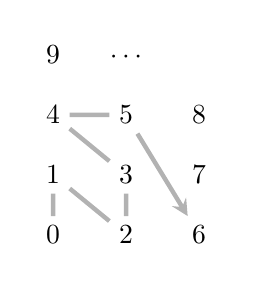
\begin{tikzpicture}
		\matrix (A) [matrix of math nodes, row sep=3mm, column sep=4mm] {
			9 & \cdots & \\
			4 & 5 & 8 \\
			1 & 3 & 7 \\
			0 & 2 & 6 \\
		};
		\draw[ultra thick, -stealth, black!30] (A-4-1) -- (A-3-1) -- (A-4-2) -- (A-3-2) -- (A-2-1) -- (A-2-2) -- (A-4-3);
	\end{tikzpicture} \qquad \begin{tikzpicture}
		\draw[->] (0,0) -- (1.5, 0) node[right] {$\aleph_0$};
		\draw[->] (0,0) -- (0, 1.5) node [above] {$\aleph_0$};
	\end{tikzpicture}\end{center}
	令序数 $\gamma$ 表 $(\aleph_\alpha \times \aleph_\alpha, \prec)$ 之序型, 并取同构 $f: \gamma \rightiso (\aleph_\alpha \times \aleph_\alpha, \prec)$. 基数的性质给出
	\[ \gamma \geq |\gamma| = |\aleph_\alpha \times \aleph_\alpha| \geq \aleph_\alpha; \]
	而 $\alpha$ 的选取蕴涵 $\gamma \neq \aleph_\alpha$, 故 $\gamma > \aleph_\alpha$. 既然 $\aleph_\alpha$ 是 $\gamma$ 的真前段, 限制 $f$ 就得到从 $\aleph_\alpha$ 至 $(\aleph_\alpha \times \aleph_\alpha, \prec)$ 的某个真前段的同构. 根据 $\prec$ 的定义, 存在序数 $\sigma < \aleph_\alpha$ 使得 $f(\aleph_\alpha) \subset \sigma \times \sigma$. 由于 $\aleph_\alpha$ 无穷, $\sigma$ 亦然.
	
	根据基数定义, 存在 $\beta < \alpha$ 使得 $|\sigma| = \aleph_\beta$. 关于 $\alpha$ 的极小性假设蕴涵 $\aleph_\beta \cdot \aleph_\beta = \aleph_\beta$. 但这么一来
	\[ \aleph_\alpha = |f(\aleph_\alpha)| \leq |\sigma| \cdot |\sigma| = \aleph_\beta \cdot \aleph_\beta = \aleph_\beta \]
	遂与 $\beta < \alpha \implies \aleph_\beta < \aleph_\alpha$ 矛盾. 证毕.
\end{proof}

\begin{corollary}\label{prop:cardinal-max}
	对任意非零基数 $\kappa$, $\lambda$, 设其一无穷, 则
	\begin{inparaenum}[(i)]
		\item $\kappa + \lambda = \kappa \cdot \lambda = \max\{\lambda, \kappa\}$;
		\item 若 $2 \leq \kappa \leq \lambda$, 则 $\kappa^\lambda = 2^\lambda$.
	\end{inparaenum}
\end{corollary}
\begin{proof}
	先证明 (i). 不妨设 $\lambda$ 无穷而且 $\lambda \geq \kappa > 0$. 基数运算的定义蕴涵
	\[ \lambda \leq \kappa + \lambda \leq \kappa \cdot \lambda \leq \lambda \cdot \lambda. \]
	鉴于 Schröder--Bernstein 定理 \ref{prop:Schröder-Bernstein}, 一切化约到证明 $\lambda = \lambda \cdot \lambda$; 为此可将 $\lambda$ 视同于某个 $\aleph_\alpha$ 并应用定理 \ref{prop:Ord2-canonical} 即可. 断言 (ii) 归结为 $2^\lambda \leq \kappa^\lambda \leq (2^{\lambda})^\lambda = 2^{\lambda \cdot \lambda} = 2^\lambda$, 因此时 $\lambda$ 必无穷.
\end{proof}

正则基数的概念将在 \S\ref{sec:Grot-universe} 派上用场, 不妨这么看: 正则基数是无法由更小的基数拼凑而成的无穷基数. \index{jishu!正则基数 (regular cardinal)}
\begin{definition}\label{def:regular-cardinal}
	一个无穷基数 $\alpha$ 称为\emph{正则基数}, 如果不存在极限序数 $\beta < \alpha$ 和严格增的序数列 $\{ a_\xi : \xi < \beta \}$ 使得 $\sup \{a_\xi : \xi < \beta\} = \alpha$.
\end{definition}

作为例子, 以下说明形如 $\aleph_{\gamma+\omega}$ 的基数均非正则, 这里 $\gamma$ 可以是任意序数: 在定义中取 $\beta := \gamma + \omega$ 和 $a_\xi := \aleph_\xi$, 关系 $\alpha := \aleph_\beta > \beta$ 理应是明显的; 而 $\aleph$ 数的定义表明 $\sup \{ a_\xi : \xi < \beta \} = \sup \{ \aleph_{\gamma + n} : n < \omega \} = \aleph_{\gamma+\omega}$.

\section{Grothendieck 宇宙}\label{sec:Grot-universe}
关于 Grothendieck 宇宙的第一手材料是 \cite[Exp.\ I, Appendice]{SGA4-1}.

\begin{definition}\index{yuzhou@宇宙 (universe)}
	本书所谓的\emph{宇宙}, 意谓一个满足下述性质的集合 $\mathcal{U}$.
	\begin{enumerate}[\bfseries {U}.1]
		\item $u \in \mathcal{U} \implies u \subset \mathcal{U}$, 即: $\mathcal{U}$ 是传递集;
		\item $u,v \in \mathcal{U} \implies \{u, v\} \in \mathcal{U}$;
		\item $u \in \mathcal{U} \implies P(u) \in \mathcal{U}$;
		\item 若 $I \in \mathcal{U}$, 一族集合 $\{u_i : i \in I\}$ 满足 $\forall i, \; u_i \in \mathcal{U}$, 则 $\bigcup_{i \in I} u_i \in \mathcal{U}$;
		\item $\Z_{\geq 0} \in \mathcal{U}$, 因此: $\emptyset \in \mathcal{U}$ (请回忆 \S\ref{sec:order} 中构造非负整数的方法).
	\end{enumerate}
	对于集合 $X$, 若 $X \in \mathcal{U}$ 则称为 $\mathcal{U}$-集; 若 $X$ 和一个 $\mathcal{U}$-集等势, 则称为 $\mathcal{U}$-小集.\index{U-ji@$\mathcal{U}$-集}
\end{definition}

给定宇宙 $\mathcal{U}$, 不难验证以下推论:
\begin{itemize}
	\item $u \subset v \in \mathcal{U} \implies u \in \mathcal{U}$;
	\item $u \in \mathcal{U} \implies \bigcup u = \bigcup_{x \in u} x  \in \mathcal{U}$;
	\item $u, v \in \mathcal{U} \implies u \times v \in \mathcal{U}$;
	\item 若 $I \in \mathcal{U}$, 一族集合 $\{u_i : i \in I\}$ 满足 $\forall i, \; u_i \in \mathcal{U}$, 则 $\prod_{i \in I} u_i \in \mathcal{U}$.
\end{itemize}

这套概念的神髓在于在 $\mathcal{U}$ 内部可以实行大部分常见的数学操作而不涉及真类, 这就为棘手的集合论问题建起一道防火墙. 然而是否有充分多、充分大的宇宙可资调用则是另一个问题, 为此我们引入以下假设.

\begin{hypothesis}[A.\ Grothendieck]\label{hyp:universe}
	对任何集合 $X$, 存在宇宙 $\mathcal{U}$ 使得 $X \in \mathcal{U}$.
\end{hypothesis}

展开相关讨论前, 不妨先勾勒集合的层垒谱系. 以超穷递归定义一族由序数枚举的集合 $V_\alpha$ 如下: \index{jihelun!层垒谱系 (cumulative hierachy)}
\begin{align*}
	V_0 & := \emptyset, \\
	V_{\alpha+1} & := P(V_\alpha), \\
	V_\alpha & :=\bigcup_{\beta < \alpha} V_\beta, \quad \text{如果 $\alpha$ 是极限序数}.
\end{align*}

不难验证每个 $V_\alpha$ 都是传递集 (定义 \ref{def:ordinal}), 并包含 $\alpha$ 作为子集, 而且 $\alpha < \beta \implies V_\alpha \subset V_\beta$.

\begin{proposition}
	任一集合都属于某个 $V_\alpha$, 其中 $\alpha$ 是序数.
\end{proposition}
\begin{proof}
	首先证明以下性质: 任何非空的类 $C$ 都有一个相对于 $\in$ 的极小元 $x$. 任取 $S \in C$. 若 $S \cap C = \emptyset$ 则 $S$ 即所求的极小元. 若 $S \cap C \neq \emptyset$, 则存在传递集 $T$ 使得 $T \supset S$, 其递归构造如下:
	\[ S_0 := S, \quad S_{n+1} := \bigcup S_n, \quad T := \bigcup_{n \in \Z_{\geq 0}} S_n; \]
	循定义可见 $T$ 是传递的. 令 $X := T \cap C$, 这是非空集故正则公理 \textbf{A.8} 确保 $X$ 中有相对于 $\in$ 的极小元 $x$. 仅须说明 $x$ 相对于 $(C, \in)$ 同样极小: 设若不然, 存在 $y \in x \cap C$, 则 $T$ 传递和 $x \in T$ 将蕴涵 $y \in T \cap C = X$, 与 $x$ 对 $(X, \in)$ 极小相悖.

	现在取 $C$ 为所有不在任一个 $V_\alpha$ 内的集合构成的类. 假设 $C$ 不空, 应用上述性质可知 $C$ 中存在一个相对于 $\in$ 的极小元 $x$. 因此若 $z \in x$ 则 $z$ 属于某个 $V_\alpha$; 对之取最小的 $\alpha = \alpha(z)$ 使得 $z \in V_\alpha$. 由于 $x$ 是集合, 应用替换公理模式 \textbf{A.7} 知 $\mathcal{O} := \{\alpha(z) : z \in x \}$ 是一个由序数组成之集合, 置 $\theta := \sup \mathcal{O}$. 于是 $x \subset V_\theta$ 故 $x \in V_{\theta+1}$, 矛盾.
\end{proof}

集合 $V_\omega$ 的元素称作遗传有限集, 这些集合皆有限, 这对于一些组合学或计算机方面的应用或许足够, 但很难想象如何在其中开展分析或几何学等理论. 因此 $V_\omega$ 对数学家是远远不够用的. Grothendieck 学派原来的定义不含 $\Z_{\geq 0} \in \mathcal{U}$, 导致 $V_0, V_\omega$ 都是它们意义下的宇宙; 本书的假设排除了这两者.

\begin{definition}\index{jishu!强不可达 (strongly inaccessible)}
	满足以下性质的基数 $\kappa$ 称为强不可达基数:
	\begin{enumerate}[\bfseries {I}.1]
		\item $\kappa$ 不可数,
		\item $\kappa$ 是正则基数 (定义 \ref{def:regular-cardinal}),
		\item 对任意基数 $\lambda$ 皆有 $\lambda < \kappa \implies 2^\lambda < \kappa$.
	\end{enumerate}
\end{definition}
可以证明 \textbf{I}.3 蕴涵 $\lambda, \nu < \kappa \implies \lambda^\nu < \kappa$, 见 \cite[p.58]{Je03}. 强不可达基数是现代集合论着力研究的大基数的一员. Bourbaki 在 \cite[Exp. I, Appendice]{SGA4-1} 中证明了以下结果.
\begin{theorem}
	宇宙正是层垒谱系中形如 $V_\kappa$ 的成员, 其中 $\kappa$ 是一个强不可达基数.
\end{theorem}

强不可达基数的性质告诉我们: 从 $V_\kappa$ 的元素出发, 在 ZFC 系统内无论怎么操作都不会超出 $V_\kappa$. 假若读者对数理逻辑有些了解, 则可以更精确地说: 对于强不可达基数 $\kappa$, 宇宙 $\mathcal{U} := V_\kappa$ 连同属于关系 $\in$ 构成了 ZFC 的一个\emph{模型} \cite[Lemma 12.13]{Je03}, 相当于在集合论内部虚拟地运行了一套集合论. 不妨这么看: 若把 $V_\kappa$ 的元素看作 ``集合'', 则就模型 $(V_\kappa, \in)$ 观之, ``类''就是 $V_{\kappa+1} = P(V_\kappa)$ 的元素.

\begin{remark}
	假设 \ref{hyp:universe} 等价于对任意基数 $\lambda$, 存在强不可达基数 $\kappa$ 使得 $\lambda < \kappa$. 这是颇强的要求. 对于大多数的范畴论构造和数学论证, 我们顶多只要求存在某个宇宙 $\mathcal{U}$; 换言之, 日常生活中只需要单个强不可达基数. 这个要求依然有些奢侈, 原因是在 ZFC 系统内无法证明强不可达基数的存在性 \cite[Theorem 12.12]{Je03}.
\end{remark}

数学工作者究竟需不需要宇宙? 如何看待强不可达基数假设? 这些议题处在数学, 哲学与群体心理学的交界, 请有兴趣的读者移步 \cite{Shu08}.

\begin{Exercises}
	\item 设 $X, Y$ 为全序集, 定义新的全序集
		\begin{compactenum}[(i)]
			\item $X \sqcup Y$, 其序结构限制到 $X$ 和 $Y$ 上分别是原给定的序, 并且对所有 $x \in X$, $y \in Y$ 都有 $x < y$;
			\item $X \times Y$, 配备反字典序: $(x_1, y_1) < (x_2, y_2)$ 当且仅当 $y_1 < y_2$, 或 $y_1=y_2$ 而 $x_1 < x_2$.
		\end{compactenum}
		证明对于序数 $\alpha, \beta$, 序数 $\alpha + \beta$ 与 $\alpha \beta$ 作为良序集分别同构于 $\alpha \sqcup \beta$ 与 $\alpha \times \beta$.
		\begin{hint} 对 $\beta$ 行超穷归纳. \end{hint}
	\item 证明序数运算的下述性质.
		\begin{compactenum}[(i)]
			\item $\beta < \gamma \implies \alpha + \beta < \alpha + \gamma$;
			\item 若 $\alpha < \beta$, 则存在唯一的 $\delta$ 使得 $\beta = \alpha + \delta$. \begin{hint} 取 $\delta$ 为良序集 $\{\xi : \alpha \leq \xi < \beta \}$;\end{hint}
			\item (带余除法) 对于 $\gamma, \alpha > 0$, 存在唯一的 $\beta, \rho$ 使得 $\rho < \alpha$ 且 $\gamma = \alpha \beta + \rho$. \begin{hint}取满足 $\alpha\beta \leq \gamma$ 的最大序数 $\beta$, 并应用 (ii); \end{hint}
			\item 若 $\alpha > 1$, 则 $\beta < \gamma \implies \alpha^\beta < \alpha^\gamma$.
		\end{compactenum}
	\item 举例说明对于序数 $\alpha, \beta$, 一般而言 $\alpha \beta \neq \beta \alpha$. \begin{hint}不妨取 $\alpha < \beta = \omega$.\end{hint}
	\item 证明任意序数 $\gamma > 0$ 皆有唯一的 Cantor 标准形
		\[ \gamma= \omega^{\alpha_1} k_1 + \cdots + \omega^{\alpha_n} k_n, \]
		其中 $n \in \Z_{\geq 1}$, $\gamma \geq \alpha_1 > \cdots > \alpha_n$ 皆为序数, 而 $k_1, \ldots, k_n \in \Z_{\geq 1}$. \begin{hint}对 $\gamma$ 作超穷递归: 取最大的 $\alpha$ 使得 $\gamma \geq \omega^\alpha $, 再用带余除法表 $\gamma = \omega^\alpha k + \rho$, 这里的 $k$ 必为有限序数. 用超穷归纳法可证唯一性.\end{hint}
	\item 证明 $f(a,b) = 2^a(2b+1)-1$ 是从 $\Z_{\geq 0} \times \Z_{\geq 0}$ 到 $\Z_{\geq 0}$ 的双射.
	\item 以下结果称作 König 引理: 设 $\kappa_i, \lambda_i$ 为两族以 $i \in I$ 为下标的基数, 且对每个 $i \in I$ 皆有 $\kappa_i < \lambda_i$. 证明
		\[ \sum_{i \in I} \kappa_i < \prod_{i \in I} \lambda_i. \]
		导出 Cantor 定理 $\kappa < 2^\kappa$ 作为特例.
		\begin{hint}
			容易看出 $\leq$ 成立. 接着取 $E := \prod_i E_i$, 其中 $|E_i| = \lambda_i$; 若断言不成立, 则存在分解 $E = \bigcup_i F_i$, 其中 $F_i \subset E$, $|F_i| = \kappa_i$. 为导出矛盾, 将每个 $f \in E$ 按分量表成 $(f_j)_{j \in I}$, $f_j \in E_j$, 并考虑集合
			\[ G_i := \Image\left[ F_i \hookrightarrow E \xrightarrow{\text{取 $i$ 分量}} E_i \right], \quad i \in I. \]
			说明 $G_i \subsetneq E_i$. 然后取 $f \in \prod_i (E_i \smallsetminus G_i)$ 并导出 $f \notin \bigcup_i F_i$, 矛盾. 这里和 Cantor 定理一样使用了对角线论证法.
		\end{hint}
\end{Exercises}


	\backmatter
	\printbibliography[heading=bibintoc, title={Daftar Pustaka}]

	{\footnotesize
	\printindex[sym1]
	\indexprologue{Istilah disusun menurut bentuk bahasa Indonesia; padanan bahasa Inggris dicantumkan bila berguna untuk penelusuran lintas bahasa.}
	\printindex
	}
\end{document}
